\documentclass[a4paper, 12pt]{article}
\usepackage[utf8]{inputenc}
\usepackage{graphicx}
\usepackage[norsk]{babel}
\usepackage{subfigure}

\begin{document}

\title{Prosjektkravspesifikasjon for Genyx}
\author{Marius Geitle}
\date{\today}

\maketitle
\tableofcontents{dsd}


\section{Introduksjon}
\subsection{Formål}
Formålet med dette dokumentet er å gi en detaljert beskrivelse av kravene til "Genyx". Det vil illustrere formålet og en komplett beskrivelse av utviklingen av systemet. Det vil også illustrere begrensningene, grensesnitt og interaksjon med ekstern programmvare. Dette dokumentet er ment for å bli presentert til Lars Emil Knudsen for godkjenning og som referanse for utvikling av første versjon.


\subsection{Omfang}
Genyx er en notat applikasjon som gjør det mulig for å benytte en android telefon for å gjøre notater under møter eller andre steder og effektivt kunne finne igjen gamle notater ved å bruke enten geografisk possisjon, tidsrom, fri-text søk, og/eller kategorisering.

Under notering vil brukeren kunne opprette et notat som består av flere sider, og sidene kan inneholde enten bilder som kan bli ikkedestruktivt annotert, tekst, eller håndtegnet grafikk slik som håndskrift eller tegninger.

Applikasjonen trenger tilgang til kaldenderprovider for å kunne knytte opp notater mot kalenderhendelser. Den trenger også tilgang til internett og både fin og grov posssisjon for geografisk markering av notater. Det vil også bli utredet om det er er hensiktsmessig å integrere med facebook for å kunne tagge notater med venner fra facebook.

\section{Overordnet beskrivelse}
\subsection{Produktperspektiv}
Applikasjonen vil være en mobil applikasjon for Android enheter. Mobilapplikasjonen blir brukt til å behandle, se, og redigere notater og behandle kategorilister.

Applikasjonen vil benytte en local SQLite database for lagring av notater, kategorilister ol.

For å tagging av notater med informasjon om hvilen kalenderhendelse dette notatet gjelder så vil applikasjonen benytte android api for tilgang til den innebygde kalenderdatabasen.

For visning av kart og geografisk tagging av notater vil en geografisk possisjonering bli utført både ved hjelp av det mobile nettverket og GPS.

Kamera vil bli benyttet for import av bilder til notater.

\subsection{produktfunksjoner}
Applikasjonen vil gjøre det mulig å opprette og redigere eksisterende notater som blir lagret i en lokal database på den mobile enheten. Notatet vil kunne bestå av flere sider som igjen er splittet opp i lag. Et lag kan bestå av bilde, kart, tekst, eller håndt-tegnet grafikk. Notater kan også inneholde bilder og andre filer som vedlegg, åpning av vedlegg vil bli benyttet av den applikasjonen på enheten som er registrert for den filtypen i systemet. Notatet kan bli merket med en eller flere kategorier, og bli merket med en geografisk posisjon. Posisjonen vil kunne merkes enten ved hjelp av manuell markering på kart, ved hjelp av mobilnett for å hente posisjon, eller ved å benytte GPS.

Med applikasjonen så vil brukeren kunne søke opp gamle notater ved hjelp av flere søkekriterier, deriblant avstand fra et punkt på et kart, fri-tekst, og kategori. Resultatene vil kunne bli vist enten på kart, eller i listeform.

Listen med kategorier som brukeren kan markere notater med vil kunne bli behandlet og det vil være mulig å slette, redigere og opprette nye kategorier.

\subsection{Brukertyper}
Denne applikasjonen vil være ment for brukere som trenger å kunne lage større notater og kunne kategoriere notatene og markere kategoriene med geografisk informasjon uten å måtte gjøre en ekstrajobb med å sette opp en ryddig struktur. Dette kan inneholde konsultener som ofte drar på møter, landskapsfotografer som ønsker når de er ute på leting etter fotosteder kan ta referansebilder og notere ned informasjon som lyssetting osv.

En annen brukergruppe er studenter som ønsker en lett app som kan bli benyttet under forelesninger for å enkelt kunne notere ned informasjon og kunne tegne av tegninger på whiteboard / tavle, men ikke ønsker å bruke tid på å sette opp mappestrukturer ol.

\subsection{Begrensninger}
Denne applikasjonen vil benytte både GPS og mobilt nett for å hente ned possisjonen til brukeren, og det kan være variasjoner i hvilke possisjonstjenester de forskjellige mobile enhetene tilbyr, og enkelte posisjonstjenester kan være utilgjenglig enkelte steder slik som GPS inne i bygninger.

Denne applikasjonen vil kreve en stor skjermstørrelse for å kunne effektivt notere ned mye informasjon.

Fordi alle data blir lagret lokalt på enheten vil antall notater som kan lagres på enheten være begrenset av tilgjenglig diskplass.

\subsection{Antagelser og avhengigheter}
En antagelse som blir tatt er at de mobile enhetene er kraftige nok, og har nok tilgjenglig ytelse til å kjøre applikasjonen.

Det er også en antagelse at alle GPS enhetene er tilgjenglig igjennom android GPS api.

\subsection{Utelating av funksjonalitet}
For å hindre at prosjektet ikke blir ferdig er det enkelt funksjonalitet som kan bli utelatt fra prosjektet. Funksjoner som kan bli utelatt er facebook integrering, og at den grafiske redigeringen av notater kan bli forenklet.

\section{Spesifikke krav}
Denne seksjonen inneholder funksjonelle krav, og en detaljert beskrivelse av systemet.

\subsection{Krav til eksterne grensesnitt}
Denne seksjonen beskriver krav til all input og output fra applikasjonen.

\subsubsection{Brukergrensesnitt}
\begin{figure}[hb]
	\centering
	\subfigure[Hjem skjerm]{%
		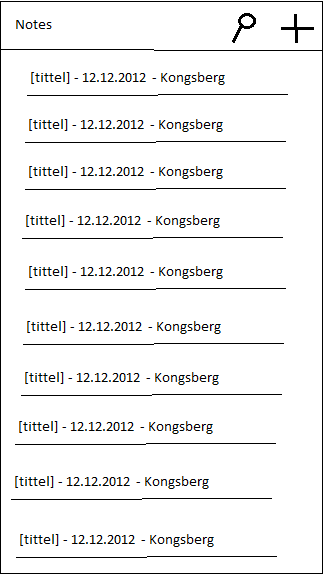
\includegraphics[width=150pt]{HomeScreen.png}
		\label{fig:homescreenfigure}}
	\quad
	\subfigure[Blush Smiley]{%
		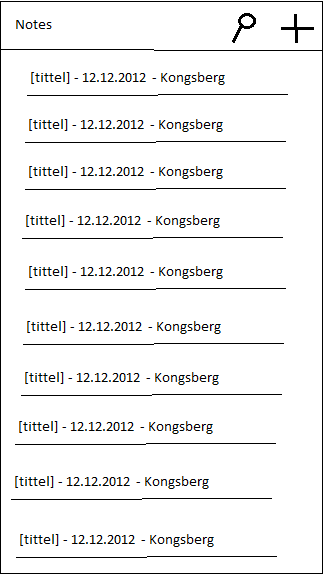
\includegraphics[width=150pt]{HomeScreen.png}
		\label{fig:subfigure2}}
	\subfigure[Sleepy Smiley]{%
		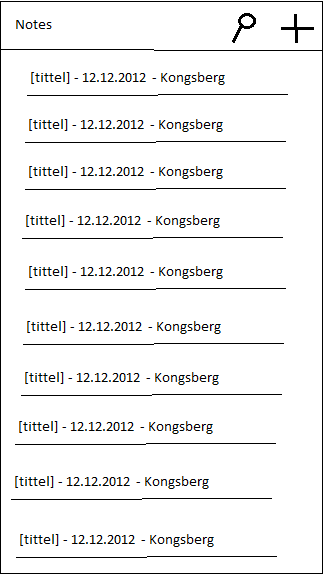
\includegraphics[width=150pt]{HomeScreen.png}
		\label{fig:subfigure3}}
	\quad
	\subfigure[Angry Smiley]{%
		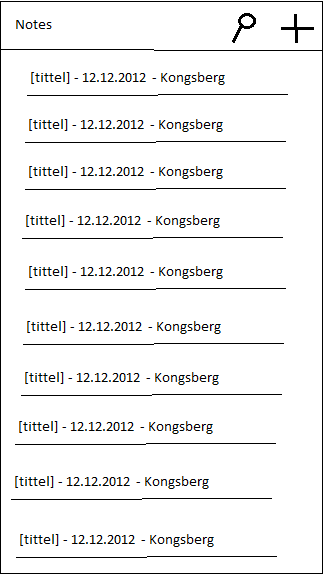
\includegraphics[width=150pt]{HomeScreen.png}
		\label{fig:subfigure4}}
	%
	\caption{Main figure caption}
\label{fig:figure}
\end{figure}

Hjemskjermen (Se Figur \ref{fig:homescreenfigure} på side~\pageref{fig:homescreenfigure}) vil inneholde en liste over alle notatene, sortert med de nyeste først. Den vil implementere lazy loading av elementer slik at ikke alle elementer lastes sammtidig. Hvert listeelement inneholder tittelen på notatet, og stedet den ble registrert (hvis tilgjenglig). og datoen den sist ble modifisert. 


\subsubsection{Maskinvaregrensesnitt}

\subsubsection{Programmvaregrensesnitt}

\subsubsection{Kommunikasjonsgrensesnitt}

\end{document}